\chapter{Klassenbeschreibung Server}

\section{Model und Dao}

\subsection{Modell der Datenbank für den Server} 

\begin{figure}[H]
	\centering
	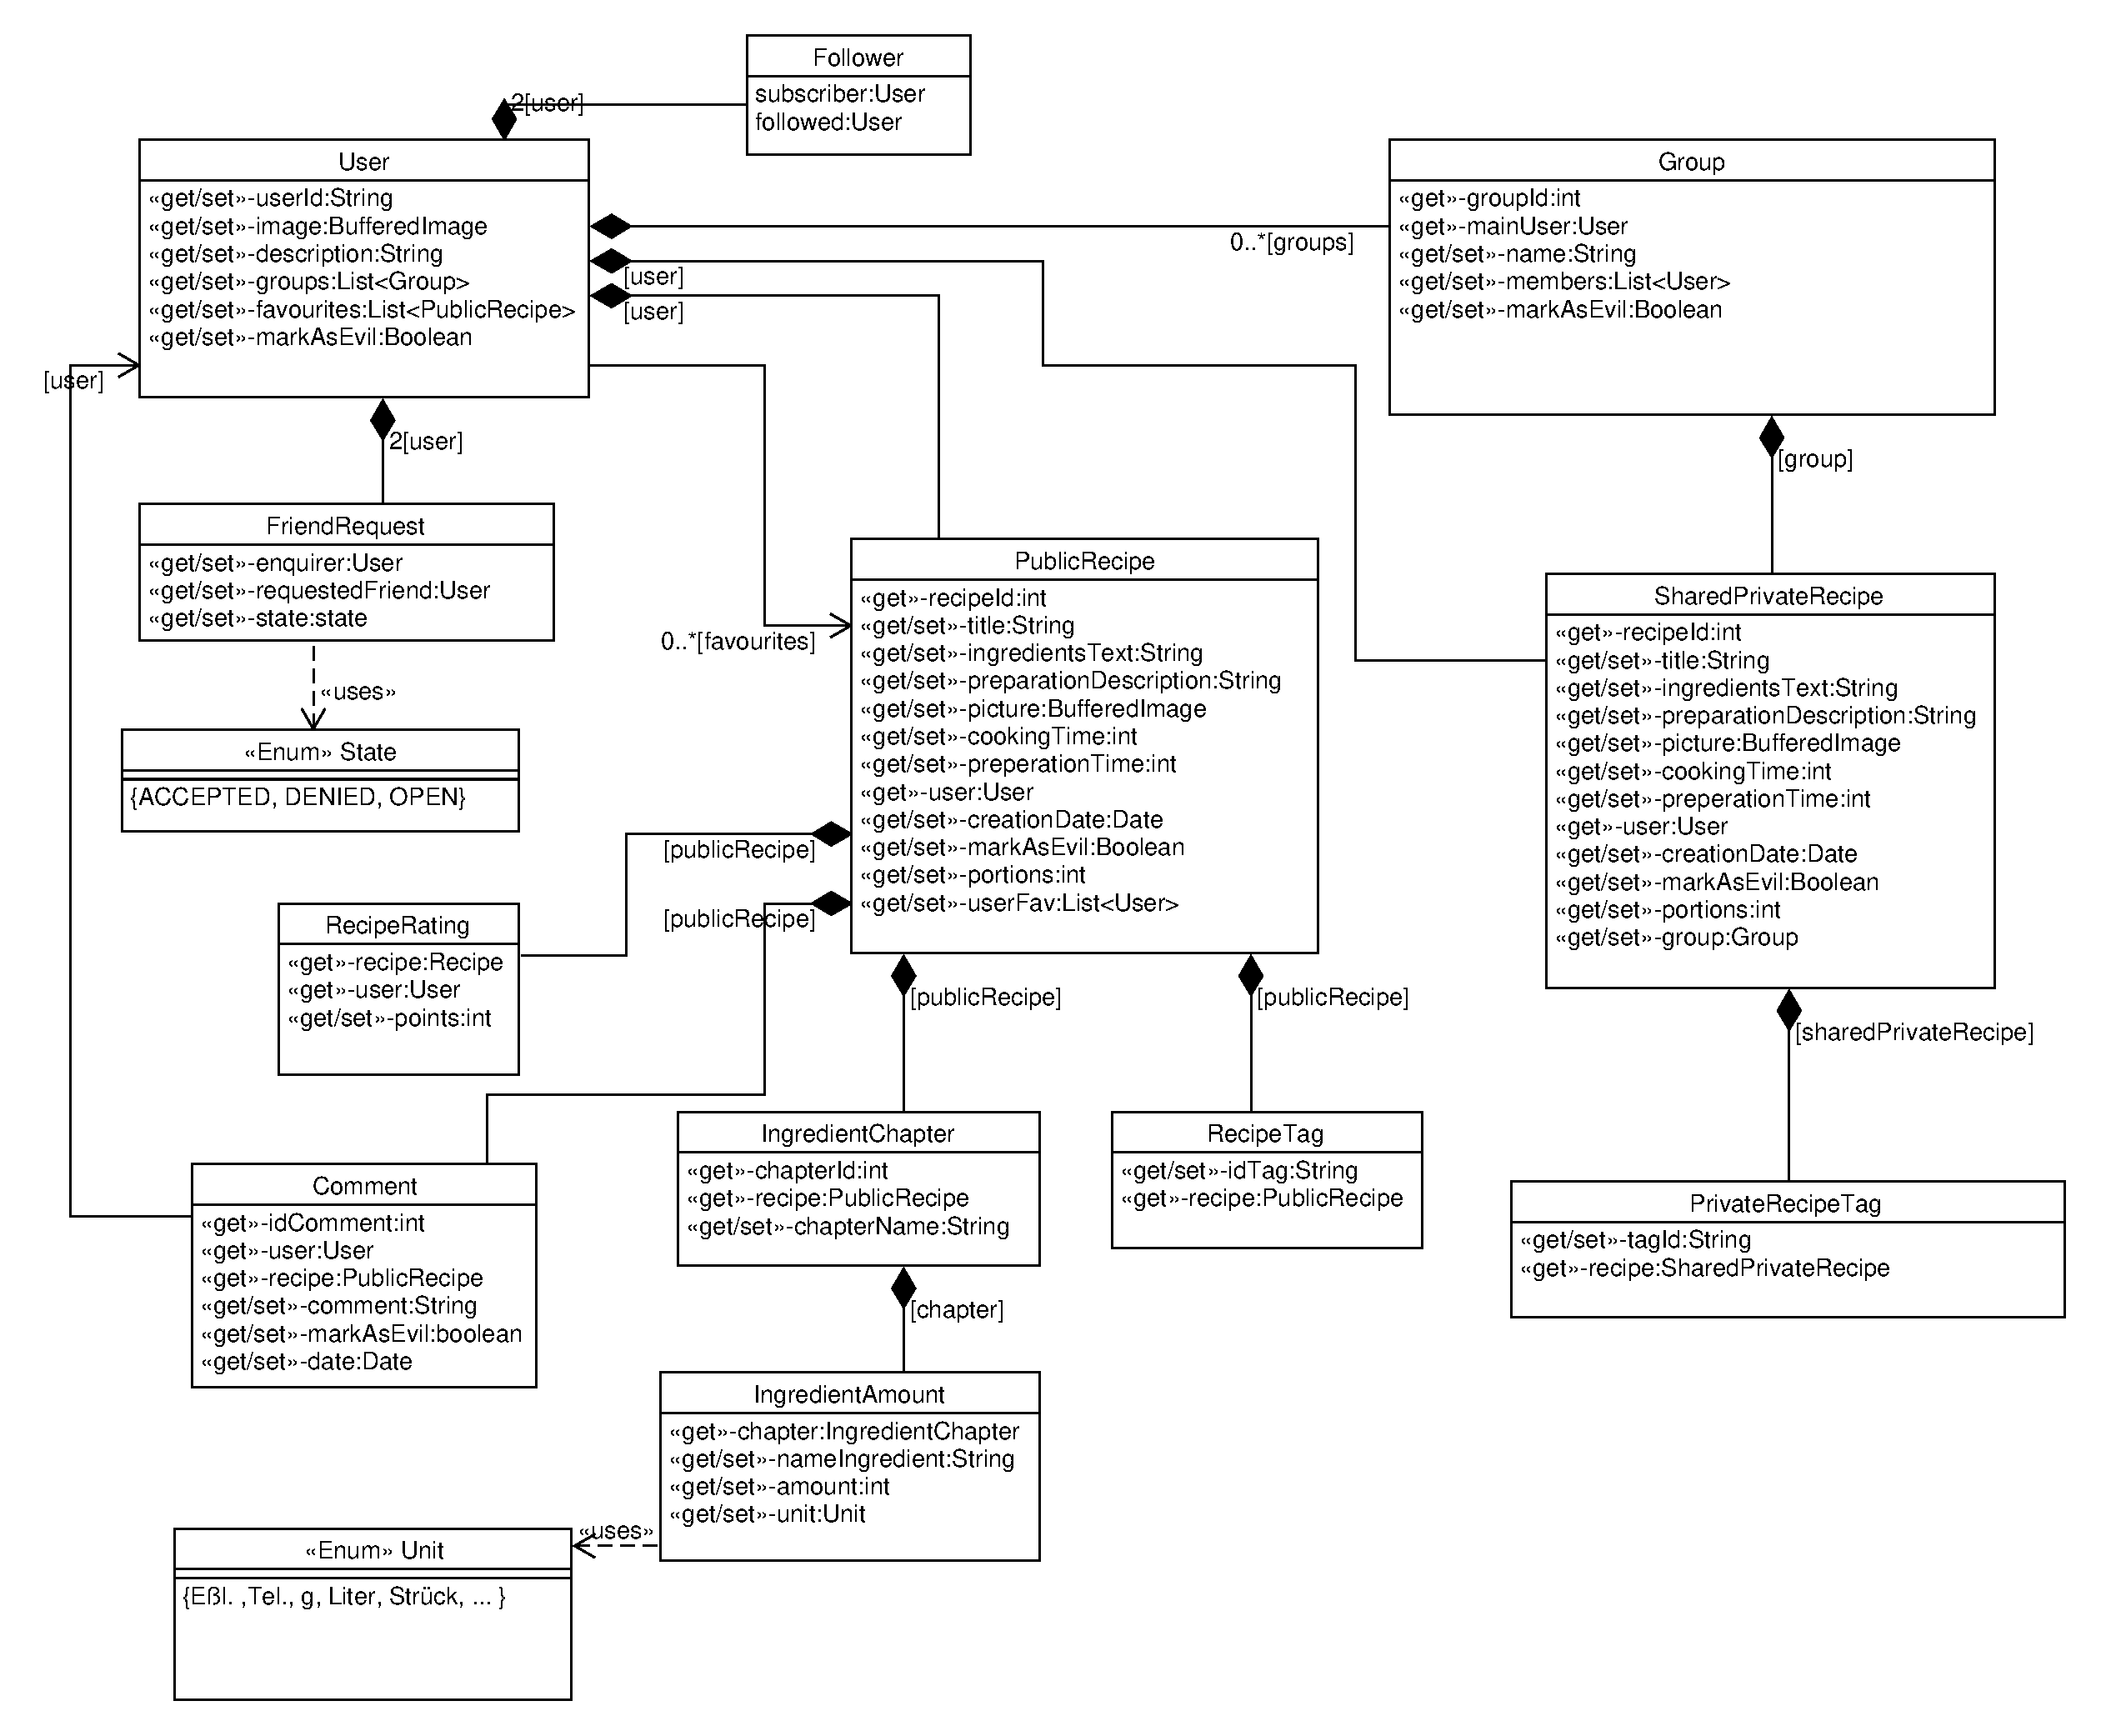
\includegraphics[width=1.0\textwidth]{pics/ServerModel.pdf}%
	\caption{Klassendiagramm für das Model für die Datenbank auf dem Server}%
\end{figure}

\subsubsection{User}
Diese Klasse beschreibt einen Nutzer der sich registriert hat.

\textbf{Attribute}
\begin{itemize}
	\item <<get/set>>-userId:String \\Die BenutzerId des Nutzers
	\item <<get/set>>-image:BufferedImage \\Profilbild des Nutzers
	\item <<get/set>>-description:String \\Personenbeschreibung des Nutzers
	\item <<get/set>>-groups:List<Group> \\Liste von Gruppen in denen sich der Nutzer befindet
	\item <<get/set>>-favourites:List<PublicRecipe> \\Liste von Rezept-Favoriten eines Nutzers
 	\item <<get/set>>-markAsEvil:Boolean \\Wird gesetzt wenn der Nutzer gemeldet wird
\end{itemize}

\subsubsection{Group}
Diese Klasse beschreibt eine Gruppe, die ein Nutzer erstellt hat.

\textbf{Attribute}
\begin{itemize}
	\item <<get>>-groupId:int \\Id der Gruppe
	\item <<get>>-mainUserId:User \\Der Nutzer, der die Gruppe erstellt hat
	\item <<get/set>>-name:String \\Name der Gruppe
	\item <<get/set>>-members:List<User> \\Liste an Nutzern die in der Gruppe sind
	\item <<get/set>>-markAsEvil:Boolean \\Wird gesetzt wenn die Gruppe gemeldet wird
\end{itemize}

\subsubsection{FriendRequest}
Diese Klasse beschreibt Freundesbeziehung zwischen zwei Nutzern.

\textbf{Attribute}
\begin{itemize}
	\item <<get/set>>-enquirer:User \\Nutzer der die Freundesanfrage stellt
	\item <<get/set>>-requestedFriend:User \\Nutzer der Angefragt wird
	\item <<get/set>>-state:state \\Status in dem sich die Anfrage befindet (ACCEPTED, DENIED, OPEN)
\end{itemize}

\subsubsection{SharedPrivateRecipe}
Diese Klasse repräsentiert ein privates Rezept das in einer Gruppe geteilt wurde.

\textbf{Attribute}
\begin{itemize}
	\item <<get>>-recipeId:int\\Eindeutige Identifikation eines öffentlichen Rezeptes
	\item <<get/set>>-title:String\\Title eines Rezeptes
	\item <<get/set>>-ingredientsText:String\\Alle Zutaten als zusammenhängender Text
	\item <<get/set>>-preparationDescription\\Zubereitungsbeschreibung eines Rezeptes
	\item <<get/set>>-picture:BufferedImage\\Bild des Gerichts
	\item <<get/set>>-cookingTime:int\\Dauer für das Kochen
	\item <<get/set>>-preperationTime:int\\Dauer für die Zubereitung
	\item <<get>>-user:User \\Nutzer der das Rezept in der Gruppe geteilt hat
	\item <<get/set>>-creationDate:Date\\Das Datum an dem das Rezept erstellt wurde
	\item <<get/set>>-markAsEvil:Boolean \\Wird gesetzt wenn das Rezept gemeldet wird
	\item <<get/set>>-portions:int\\Anzahl für wie viel Personen das Rezept gedacht ist
	\item <<get/set>>-group:Group \\Gruppe in der sich das Rezept befindet
\end{itemize}

\subsubsection{PrivateRecipeTag}
Diese Klasse repräsentiert ein Tag für ein Rezept.

\textbf{Attribute}
\begin{itemize}
	\item <<get/set>>-tagId:String \\Name des Tags
	\item <<get/>>-recipe:SharedPrivateRecipe \\Rezepte zu dem der Tag zugewiesen ist
\end{itemize}

\subsubsection{PublicRecipe}
Diese Klasse beschreibt ein öffentliches Rezept, welches von der Datenbank geladen oder gespeichert wird.

\textbf{Attribute}
\begin{itemize}
	\item <<get>>-recipeId:int\\Eindeutige Identifikation eines öffentlichen Rezeptes
	\item <<get/set>>-title:String\\Title eines Rezeptes
	\item <<get/set>>-ingredientsText:String\\Alle Zutaten als zusammenhängender Text
	\item <<get/set>>-preparationDescription\\Zubereitungsbeschreibung eines Rezeptes
	\item <<get/set>>-picture:BufferedImage\\Bild des Gerichts
	\item <<get/set>>-cookingTime:int\\Dauer für das Kochen
	\item <<get/set>>-preperationTime:int\\Dauer für die Zubereitung
	\item <<get>>-user:User\\Nutzers, dem das Rezept gehört
	\item <<get/set>>-creationDate:Date\\Das Datum an dem das Rezept erstellt wurde
	\item <<get/set>>-markAsEvil:Boolean \\Wird gesetzt wenn das Rezept gemeldet wird
	\item <<get/set>>-portions:int\\Anzahl für wie viel Personen das Rezept gedacht ist
	\item <<get/set>>-userFav:List<User> \\Nutzer die das Rezept favorisiert haben
\end{itemize}

\subsubsection{RecipeRating}
Diese Klasse repräsentiert ein Bewertung für ein Rezept.

\textbf{Attribute}
\begin{itemize}
	\item <<get>>-recipe:Recipe \\Rezept zu dem die Bewertung gehört
	\item <<get>>-user:User \\Nutzer der die Bewertung abgegeben hat
	\item <<get/set>>-points:int \\Punkte die ein Nutzer zu dem Rezept gegeben hat
\end{itemize}

\subsubsection{Comment}
Diese Klasse repräsentiert ein Kommentar für ein Rezept.

\textbf{Attribute}
\begin{itemize}
	\item <<get>>-idComment:int \\Id des Kommentars
	\item <<get>>-user:User \\Nutzer der den Kommentar erstellt hat
	\item <<get>>-recipe:PublicRecipe \\Rezept zu dem der Kommentar zugewiesen ist
	\item <<get/set>>-comment:String \\Text des Kommentares
	\item <<get/set>>-markAsEvil:Boolean \\Wird gesetzt wenn der Kommentar gemeldet wird
	\item <<get>>-date:Date \\Datum wann der Kommentar erstellt wurde
\end{itemize}

\subsubsection{PublicRecipeTag}
Diese Klasse repräsentiert ein Tag für ein Rezept.

\textbf{Attribute}
\begin{itemize}
	\item <<get/set>>-tagId:String \\Name des Tags
	\item <<get/>>-recipe:PublicRecipe \\Rezept zu dem der Tag zugewiesen ist
\end{itemize}

\subsubsection{IngredientChapter}
Diese Klasse repräsentiert ein Kapitel von den Zutaten für ein Rezept.

\textbf{Attribute}
\begin{itemize}
	\item <<get>>-chapterId:int \\Die Id des Kapitels
	\item <<get>>-recipe:PublicRecipe \\Rezept zu dem ein Kapitel zugewiesen ist
	\item <<get/set>>-ingredientChapterTitle:String \\Der Titel des Kapitels
\end{itemize}

\subsubsection{IngredientAmount}
Diese Klasse repräsentiert eine Zutat von einem Kapitel für ein Rezept.

\textbf{Attribute}
\begin{itemize}
	\item <<get>>-chapter:IngredientChapter \\Kapitel zu dem die Zutat zugeordnet ist
	\item <<get/set>>-nameIngredient:String \\Name der Zutat
	\item <<get/set>>-amount:int \\Menge der Zutat
	\item <<get/set>>-unit:String \\Einheit der Zutat (Eßl. ,Tel., g, Liter, Strück, ... )
\end{itemize}

\subsection{Dao der Datenbank für den Server} 

\begin{figure}[H]
	\centering
	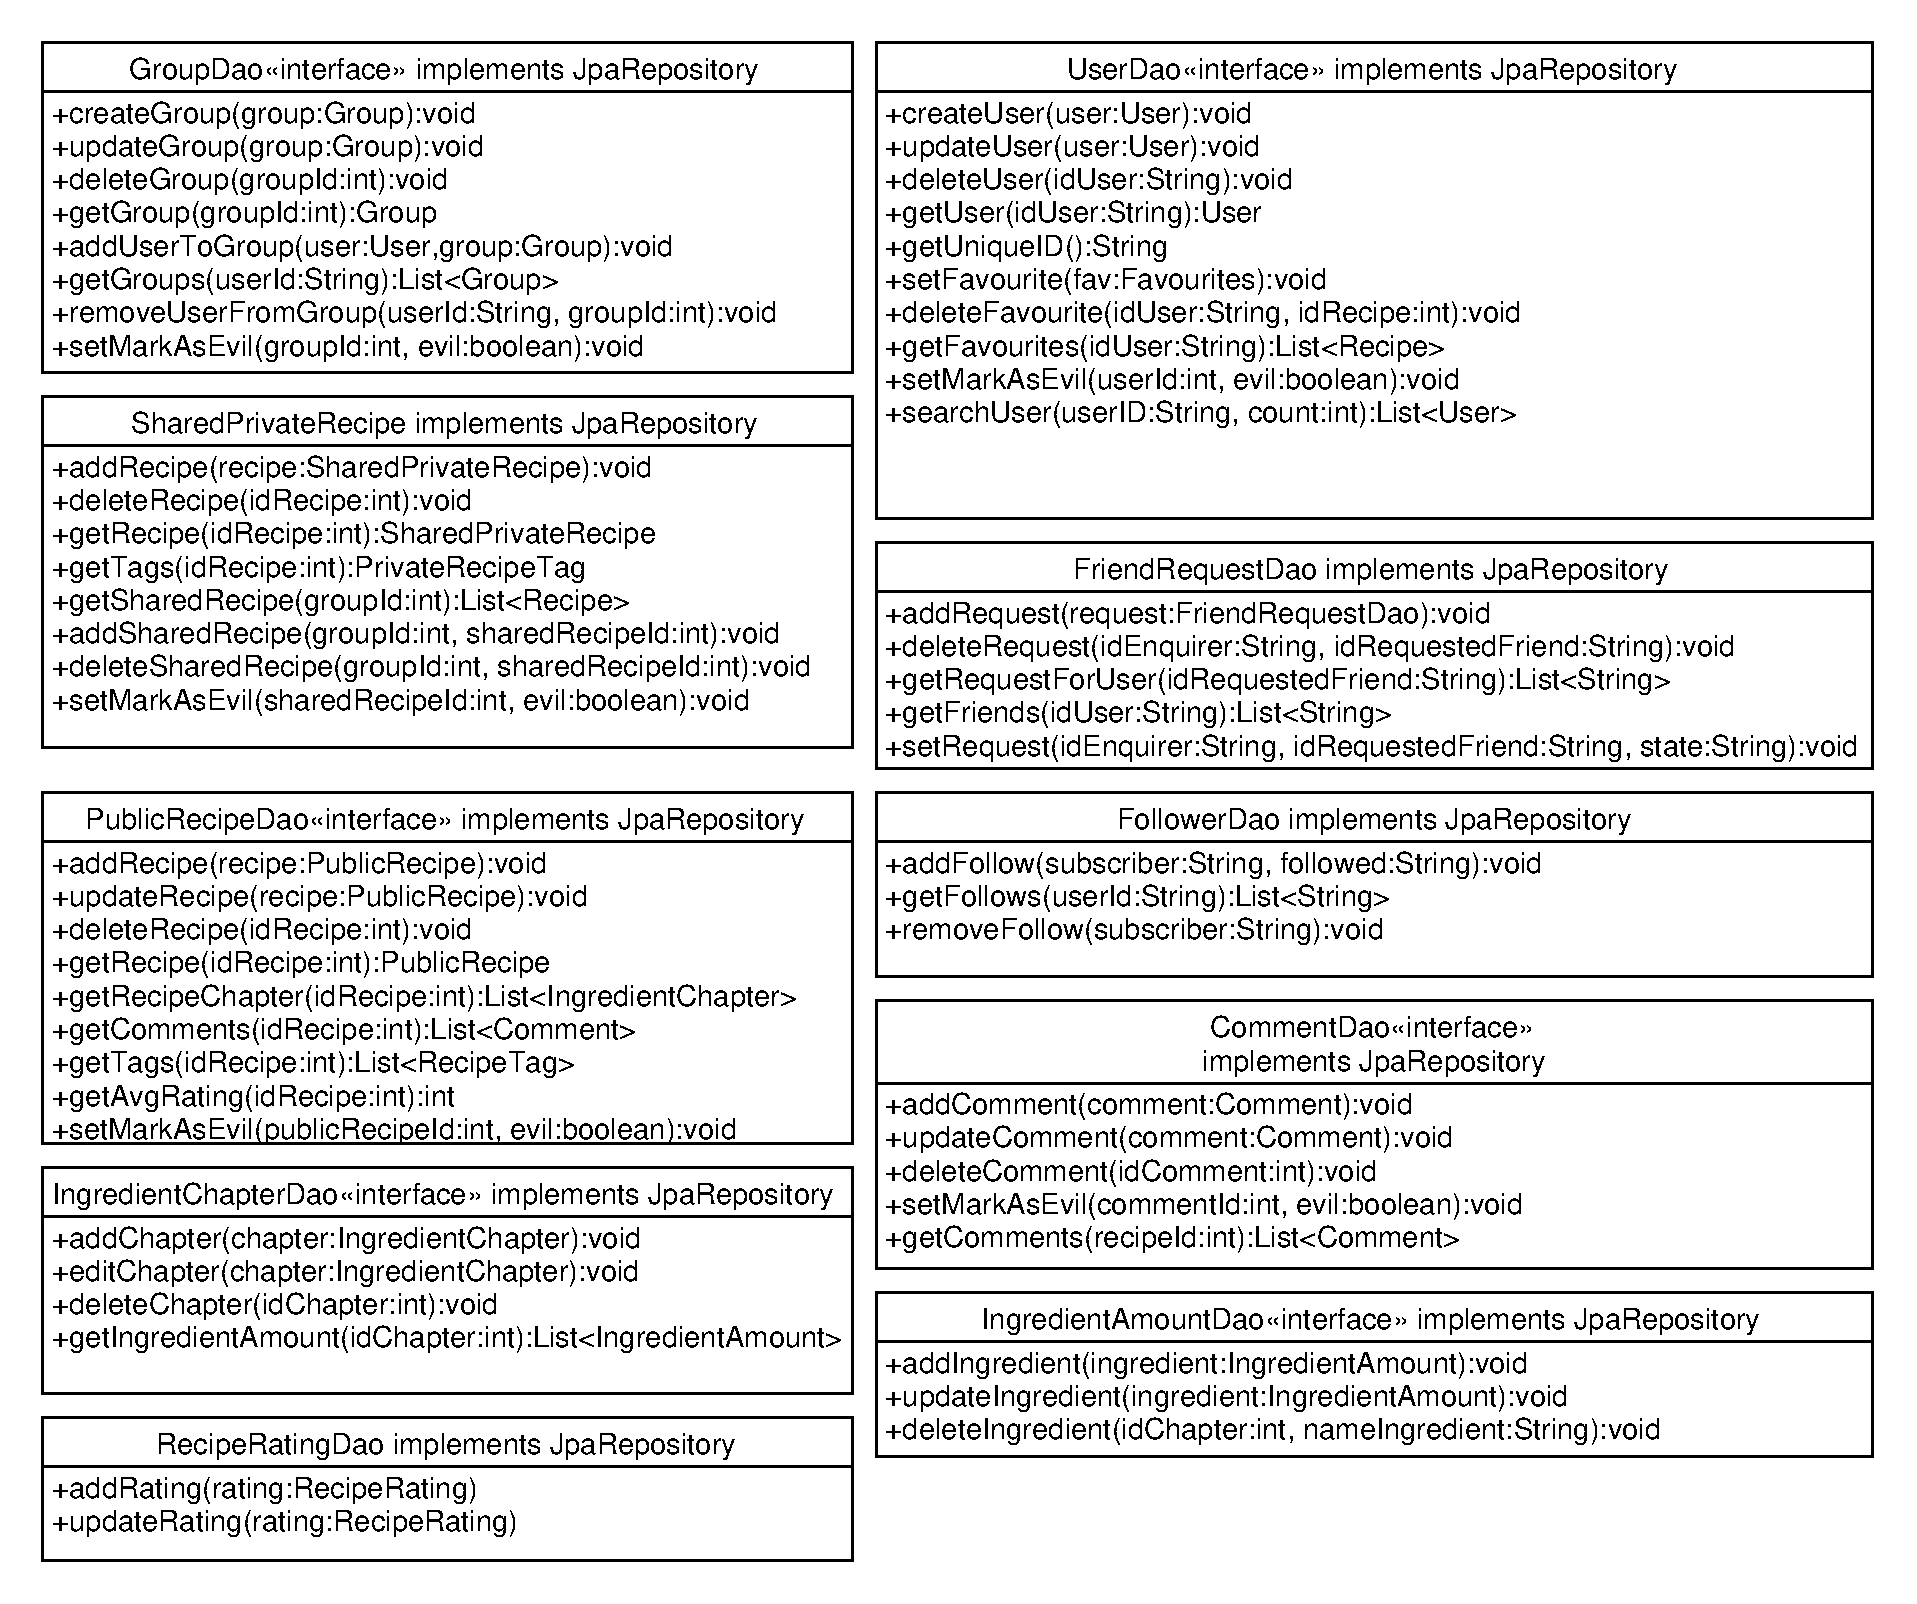
\includegraphics[width=0.7\textwidth]{pics/ServerDaos.pdf}%
	\caption{Klassendiagramm für die Daos für den Datenbankzugriff auf dem Server}%
\end{figure}

\subsubsection{GroupDao<<interface>>}
Diese Klasse gibt Schnittstellen für Gruppen in der Datenbank an.

\textbf{Methoden}
\begin{itemize}
	\item +createGroup(group:Group):void \\Fügt die übergebene Gruppe hinzu
	\item +updateGroup(group:Group):void \\Aktualisiert  einen Eintrag mit der übergebenen Gruppe
	\item +deleteGroup(groupId:int):void \\Löscht eine Gruppe mit der entsprechenden Id
	\item +getGroup(groupId:int):Group \\Gibt die Gruppe mit der entsprechenden Id zurück
	\item +addUserToGroup(user:User,group:Group):void \\Fügt einen Nutzer einer Gruppe hinzu
	\item +getGroups(userId:String):List<Group> \\Gibt die Gruppen eines Nutzers zurück
	\item +removeUserFromGroup(userId:String, groupId:int):void \\Entfernt einen Nutzer von einer Gruppe
	\item +setMarkAsEvil(groupId:int, evil:boolean):void \\Setzt den Zustand, wenn eine Gruppe gemeldet wurde
\end{itemize}

\subsubsection{UserDao<<interface>>}
Diese Klasse gibt Schnittstellen für Nutzer in der Datenbank an.

\textbf{Methoden}
\begin{itemize}
	\item +createUser(user:User):void \\Fügt den übergebenen Nutzer hinzu
	\item +updateUser(user:User):void \\Aktualisiert einen Nutzer mit dem übergebenen Nutzer
	\item +deleteUser(idUser:String):void \\Löscht einen Nutzer mit der entsprechenden Id
	\item +getUser(idUser:String):User \\Gibt einen Nutzer mit der entsprechenden Id zurück
	\item +getUniqueID():String \\Gibt eine Eindeutige Id für einen Nutzer zurück
	\item +setFavourite(fav:Favourites):void \\Fügt ein Favorit hinzu
	\item +deleteFavourite(idUser:String, idRecipe:int):void \\Löscht einen Favoriten
	\item +getFavourites(idUser:String):List<Recipe> \\Gibt die Liste an Favoriten von einem Nutzer zurück
	\item +setMarkAsEvil(userId:int, evil:boolean):void \\Setzt den Zustand, wenn ein Nutzer gemeldet wurde
	\item +searchUser(userID:String, count:int):List<User> \\Sucht bestimmte Nutzer mit der übergebenen Id
\end{itemize}

\subsubsection{SharedPrivateRecipeDao<<interface>>}
Diese Klasse gibt Schnittstellen für die SharedPrivateRecipes in der Datenbank an.

\textbf{Methoden}
\begin{itemize}
	\item +addRecipe(recipe:SharedPrivateRecipe):void \\Fügt ein neues geteiltes privates Rezept hinzu
	\item +deleteRecipe(idRecipe:int):void \\Löscht ein Rezept mit der entsprechenden Id
	\item +getRecipe(idRecipe:int):SharedPrivateRecipe \\Gibt ein Rezept mit der entsprechenden Id zurück
	\item +getTags(idRecipe:int):PrivateRecipeTag \\Gibt die Liste von Tags eines Rezeptes zurück
	\item +getSharedRecipe(groupId:int):List<Recipe> \\Gibt eine Liste von Rezepten von einer Gruppe mit der entsprechenden Id zurück
	\item +addSharedRecipe(groupId:int, sharedRecipeId:int):void \\Fügt ein geteiltes privates Rezept einer Gruppe hinzu
	\item +deleteSharedRecipe(groupId:int, sharedRecipeId:int):void \\Entfernt ein Rezept von einer Gruppe
	\item +setMarkAsEvil(sharedRecipeId:int, evil:boolean):void \\Setzt den Zustand, wenn ein geteiltes private Rezept gemeldet wurde
\end{itemize}

\subsubsection{FriendRequestDao<<interface>>}
Diese Klasse gibt Schnittstellen für die Freundschaftsanfragen in der Datenbank an.

\textbf{Methoden}
\begin{itemize}
	\item +addRequest(request:FriendRequestDao):void \\Fügt die übergebene Anfrage hinzu
	\item +deleteRequest(idEnquirer:String, idRequestedFriend:String):void \\Löscht die übergebene Anfrage
	\item +getRequestForUser(idRequestedFriend:String):List<String> \\Gibt eine Liste von Nutzern, die einen Nutzer angefragt haben
	\item +getFriends(idUser:String):List<String> \\Gibt die Liste an Freunden eines Nutzers zurück
	\item +setRequest(idEnquirer:String, idRequestedFriend:String, state:String):void \\Setzt den Status einer Anfrage
\end{itemize}

\subsubsection{PublicRecipeDao<<interface>>}
Diese Klasse gibt Schnittstellen für die öffentlichen Rezepte in der Datenbank an.

\textbf{Methoden}
\begin{itemize}
	\item +addRecipe(recipe:PublicRecipe):void \\Fügt das übergebene öffentliche Rezept hinzu
	\item +updateRecipe(recipe:PublicRecipe):void \\Aktualisiert ein Rezept mit dem übergebenen Rezept
	\item +deleteRecipe(idRecipe:int):void \\Löscht ein Rezept mit der entsprechenden Id
	\item +getRecipe(idRecipe:int):PublicRecipe \\Gibt ein Rezept mit der entsprechenden Id zurück
	\item +getRecipeChapter(idRecipe:int):List<IngredientChapter> \\Gibt eine Liste von Kapiteln von einem Rezept mit der entsprechenden Id zurück
	\item +getComments(idRecipe:int):List<Comment> \\Gibt eine Liste von Kommentaren von einem Rezept mit der entsprechenden Id zurück
	\item +getTags(idRecipe:int):List<RecipeTag> \\Gibt die Tags eines Rezeptes mit der entsprechenden Id zurück
	\item +getAvgRating(idRecipe:int):int \\Gibt die Druchschnittsbewertung eines Rezeptes zurück
	\item +setMarkAsEvil(publicRecipeId:int, evil:boolean):void \\Setzt den Zustand, wenn ein Rezept gemeldet wurde
\end{itemize}

\subsubsection{FollowerDao<<interface>>}
Diese Klasse gibt Schnittstellen für Follow-Einträge in der Datenbank an.

\textbf{Methoden}
\begin{itemize}
	\item +addFollow(subscriber:String, followed:String):void \\Fügt ein neuer Eintrage für einen Follow ein
	\item +getFollows(userId:String):List<String> \\Gibt eine Liste von Nutzern zurück, die der Nutzer folgt
	\item +removeFollow(subscriber:String):void \\Löscht einen Eintrag in der Tabelle mit den entsprechenden Nutzern
\end{itemize}

\subsubsection{CommentDao<<interface>>}
Diese Klasse gibt Schnittstellen für Kommentaren von Rezepten in der Datenbank an.

\textbf{Methoden}
\begin{itemize}
	\item +addComment(comment:Comment):void \\Fügt ein neuen Kommentar einem Rezept hinzu
	\item +updateComment(comment:Comment):void \\Aktualisiert einen Kommentar
	\item +deleteComment(idComment:int):void \\Löscht einen Kommentar mit der entsprechenden Id
	\item +setMarkAsEvil(commentId:int, evil:boolean):void \\Setzt den Zustand, wenn ein Kommentar gemeldet wurde
	\item +getComments(recipeId:int):List<Comment> \\Gibt eine Liste von Kommentaren von einem Rezept zurück
\end{itemize}

\subsubsection{IngredientChapterDao<<interface>>}
Diese Klasse gibt Schnittstellen für Kapitel von Rezepten in der Datenbank an.

\textbf{Methoden}
\begin{itemize}
	\item +addChapter(chapter:IngredientChapter):void \\Fügt ein neues Kapitel einem Rezept hinzu
	\item +editChapter(chapter:IngredientChapter):void \\Editiert ein Kapitel
	\item +deleteChapter(idChapter:int):void \\Löscht ein Kapitel mit der entsprechenden Id
	\item +getIngredientAmount(idChapter:int):List<IngredientAmount> \\Gibt eine Liste von Zutaten von einem Kapitel zurück
\end{itemize}

\subsubsection{IngredientAmountDao<<interface>>}
Diese Klasse gibt Schnittstellen für Zutaten von Kapiteln in der Datenbank an.

\textbf{Methoden}
\begin{itemize}
	\item +addIngredient(ingredient:IngredientAmount):void \\Fügt ein neue Zutat einem Kapitel hinzu
	\item +updateIngredient(ingredient:IngredientAmount):void \\Aktualisiert eine Zutat von einem Kapitel
	\item +deleteIngredient(idChapter:int, nameIngredient:String):void \\Löscht eine Zutat von einem Kapitel
\end{itemize}

\subsubsection{RecipeRatingDao<<interface>>}
Diese Klasse gibt Schnittstellen für Bewertungen von Rezepten in der Datenbank an.

\textbf{Methoden}
\begin{itemize}
	\item +addRating(rating:RecipeRating) \\Fügt eine Bewertung hinzu von einem Rezept
	\item +updateRating(rating:RecipeRating) \\Aktualisiert eine Bewertung von einem Rezept
\end{itemize}

% Server Datenbank Section
\section{Datenbank}

\subsection{ServerDatenbank}

\begin{sidewaysfigure}[ht]
	\centering
	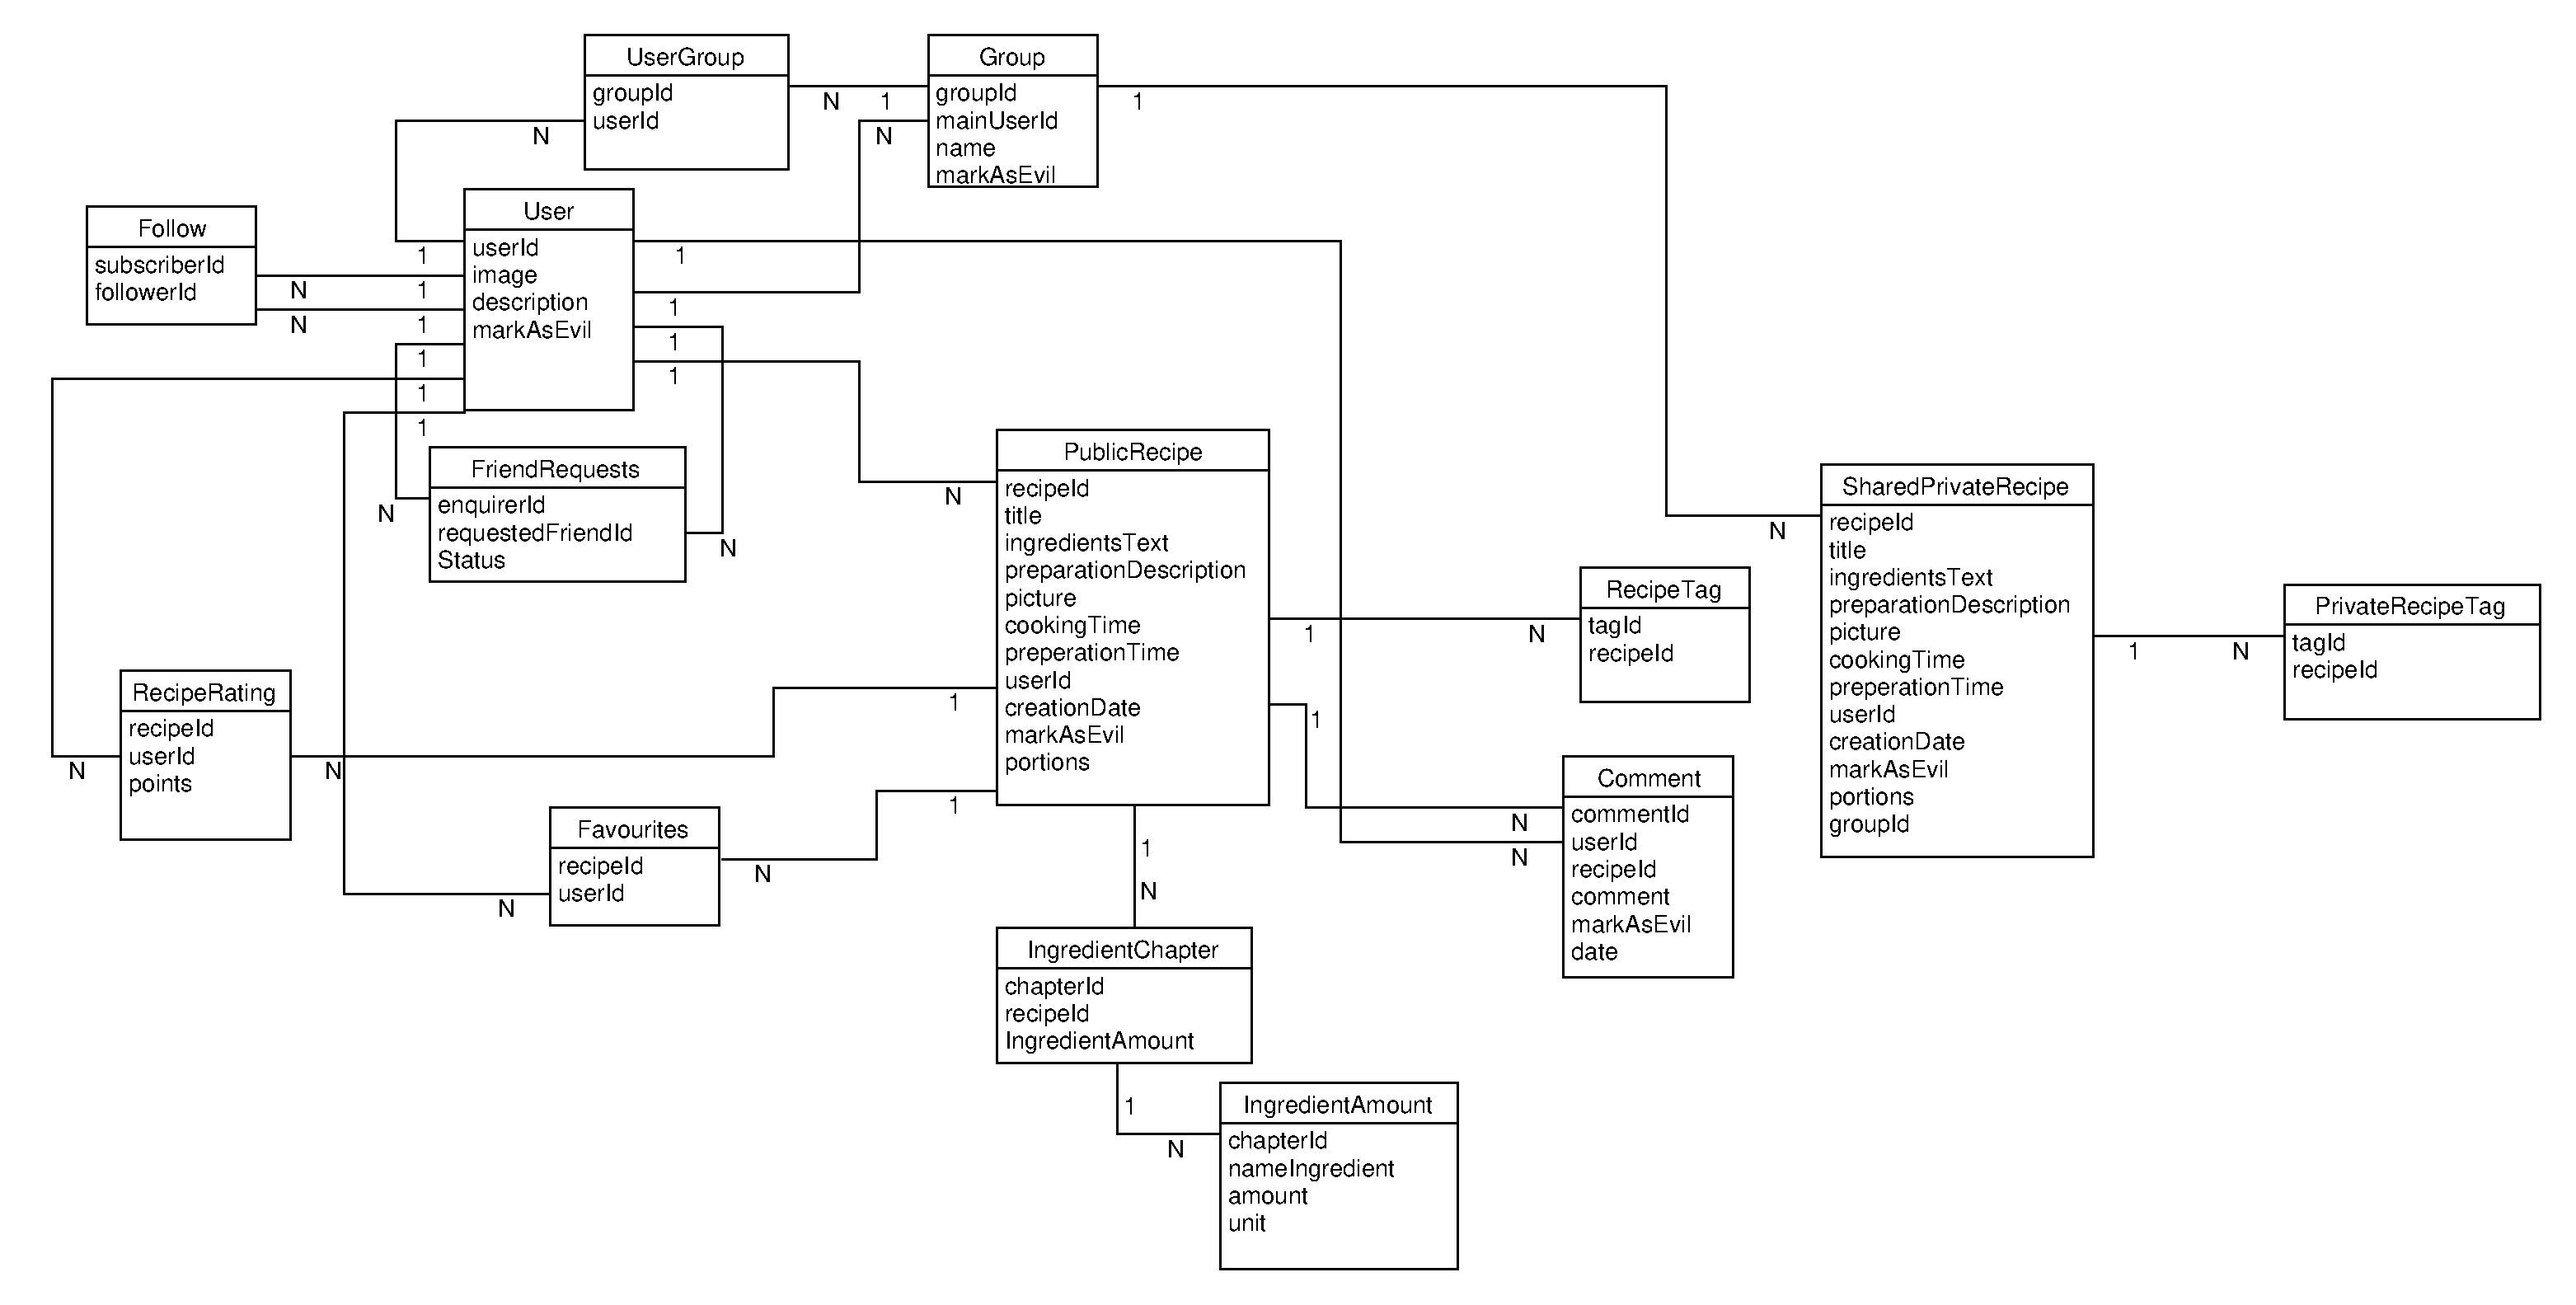
\includegraphics[width=1.0\textwidth]{pics/ServerDB.pdf}%
	\caption{ER-Diagramm der Serverdatenbank}%
\end{sidewaysfigure}

\textbf{User}\\
Die Relation User beinhaltet Informationen über die Profile der angemeldeten Nutzer. Die Relation User wird über einen Fremdschlüssel in den Relationen UserGroup, Group, SharedPrivateRecipe, PublicRecipe, Favourites, RecipeRating und FriendRequests adressiert.

\begin{itemize}
 	\item userId \\ Eindeutige Kennung eines angemeldeten Nutzers, mit dem er sich anmeldet (Primärschlüssel)
 	\item image \\ Profilbild der Nutzers
 	\item description \\ Textuelle Beschreibung des Profils
 	\item markAsEvil \\ Markiert gemeldete Nutzer
\end{itemize}

\textbf{FriendRequest}\\
Die Relation FriendRequest beinhaltet Informationen über noch ausstehende Freundschaftsanfragen. Die Relation FriendRequest verweist selbst auf die Relation User.

\begin{itemize}
	\item enquirerId \\ BenutzerID des anfragenden Nutzers (Fremdschlüssel)
	\item requestedFriendId \\ BenutzerID des angefragten Nutzers (Fremdschlüssel)
	\item Status %macht das Sinn? Wenn eine Anfrage angenommen wird, kann man diese doch dann direkt in die Feundestabelle eintragen
\end{itemize}

\textbf{Group}\\
Die Relation Group beinhaltet Informationen über Freundesgruppen. Die Relation Group verweist auf die Relation User.

\begin{itemize}
	\item groupId \\ Eindeutige Kennung einer Gruppe (Primärschlüssel)
	\item mainUserId \\ BenutzerID des Erstellers der Gruppe (Fremdschlüssel)
	\item name \\ Name der Gruppe
	\item markAsEvil \\ Markiert gemeldete Gruppen
\end{itemize}

\textbf{UserGroup}\\
Die Relation UserGroup weist den Freundesgruppen jeweils die Mitglieder zu. Die Relation UserGroup verweist selbst auf die Relation Group und User.

\begin{itemize}
	\item groupId \\ definiert um welche Gruppe es sich handelt (Fremdschlüssel)
	\item userId \\ BenutzerID, welcher in der Gruppe mit groupId ist
\end{itemize}

\textbf{SharedPrivateRecipe}\\
Die Relation SharedPrivateRecipe beinhaltet Informationen über geteilte private Rezepte in Freundesgruppen. Die Relation SharedPrivateRecipe verweist über groupId zu einer Gruppe und verweist selbst auf die Relation User.

\begin{itemize}
	\item recipeId \\ Eindeutige Kennung des Rezeptes in dieser Tabelle (Primärschlüssel)
	\item title \\ Titel des Rezeptes
	\item ingredientsText \\ Textuelle Beschreibung der Zutaten
	\item preparationDescription \\ Textuelle Beschreibung der Zubereitung
	\item picture \\ Bild des Rezeptes
	\item cookingTime \\ Dauer der Kochzeit in Minuten
	\item preparationTime \\ Dauer der Vorbereitung in Minuten
	\item userId \\ BenutzerID des Benutzers, der dieses Rezept geteilt hat (Fremdschlüssel)
	\item creationDate \\ Datum und Uhrzeit der Versendung des Rezeptes
	\item markAsEvil \\ Markiert gemeldete Rezepte
	\item portions \\ Anzahl Portionen für die das Rezept ausgelegt ist
	\item groupId \\ Verlinkung zu welcher Gruppe das Rezept gehört
\end{itemize}

\textbf{PrivateRecipeTag}\\
Die Relation PrivateRecipeTag weist jedem privaten Rezept, welches in einer Freundesgruppe geteilt wurde, eine Menge an Tags zu. Die Relation PrivateRecipeTag verweist selbst auf die Relation SharedPrivateRecipe.

\begin{itemize}
	\item tagId \\ Name des Tags %würde es nur name nennen, da idTag impliziert, dass es sich um einen Primärschlüssel handelt und das ist es nicht
	\item recipeId \\ Rezept, zu dem der Tag gehört (Fremdschlüssel)
\end{itemize}


\textbf{PublicRecipe}\\
Die Relation PublicRecipe beinhaltet Informationen über veröffentlichte Rezepte. Die Relation PublicRecipe wird über einen Fremdschlüssel in den Relationen RecipeRating, Favourites, IngredientChapter, Comment, RecipeTag und SharedPrivateRecipe adressiert und verweist selbst auf die Relation User.

\begin{itemize}
	\item recipeId \\ Eindeutige Kennung eines Rezeptes (Primärschlüssel)
	\item title \\ Titel des Rezeptes
	\item ingredientsText \\ Textuelle Beschreibung der Zutaten
	\item preparationDescription \\ Textuelle Beschreibung der Zubereitung
	\item picture \\ Bild des Rezeptes
	\item cookingTime \\ Dauer der Kochzeit in Minuten
	\item preparationTime \\ Dauer der Vorbereitung in Minuten
	\item userId \\ BenutzerID des Benutzers, der dieses Rezept geteilt hat (Fremdschlüssel)
	\item creationDate \\ Datum und Uhrzeit der Veröffentlichung des Rezeptes
	\item markAsEvil \\ Markiert gemeldete Rezepte
	\item portions \\ Anzahl Portionen für die das Rezept ausgelegt ist
\end{itemize}



\textbf{RecipeTag}\\
Die Relation RecipeTag weist jedem veröffentlichten Rezept eine Menge an Tags zu. Die Relation RecipeTag verweist selbst auf die Relation PublicRecipe.

\begin{itemize}
	\item tagId \\ Name des Tags %würde es nur name nennen, da idTag impliziert, dass es sich um einen Primärschlüssel handelt und das ist es nicht
	\item recipeId \\ Rezept, zu dem der Tag gehört (Fremdschlüssel)
\end{itemize}

\textbf{Comment}\\
Die Relation Comment weist jedem veröffentlichten Rezept eine Menge an Kommentaren zu. Die Relation Comment verweist selbst auf die Relationen und User und PublicRecipe.

\begin{itemize}
	\item commentId \\ Eindeutige Kennung des Kommentars
	\item userId \\ Nutzer, der den Kommentar geschrieben hat
	\item recipeId \\ Rezept, zu welchem der Kommentar gehört
	\item commit \\ Der eigentliche Kommentar
	\item markAsEvil \\ Markiert gemeldete Kommentare
	\item date \\Das Datum wann der Kommentar stellt wurde
%Man benötigt doch sicherlich einen Timestamp? Die Kommentare sollen ja chronologisch geordnet werden.
\end{itemize}

\textbf{IngredientChapter}\\
Die Relation IngredientChapter weist jedem veröffentlichten Rezept eine Menge an Unterkapiteln der Zutatenliste zu. Die Relation IngredientChapter wird über einen Fremdschlüssel in der Relation IngredientAmount adressiert und verweist selbst auf die Relation PublicRecipe.

\begin{itemize}
	\item chapterId \\ Eindeutige Kennung des Unterkapitels
	\item recipeId \\ Zeiger auf das Rezept
	\item ingredientAmount 
\end{itemize}
% bin mir nicht ganz sicher was ingredientAmount ist, aber müsste nicht noch der Name des Kapitels gespeichert werden?

\textbf{IngredientAmount}\\
Die Relation IngredientAmount weist einem Unterkapitel der Zutatenliste eines veröffentlichten Rezeptes eine Menge an Zutaten zu. Die Relation IngredientAmount verweist selbst auf die Relation IngredientChapter.

\begin{itemize}
	\item chapterId \\ Zeiger auf das Unterkapitel
	\item nameIngredient \\ Name der Zutat
	\item unit \\ Einheit, in der die Zutat gemessen wird
	\item amount \\ Anzahl an unit in der die Zutat benötigt wird
\end{itemize}

\textbf{Favourites}\\
Die Relation Favourites weist jedem angemeldeten Nutzer eine Menge an von ihm favorisierten Rezepten zu. Die Relation Favourites verweist selbst auf die Relationen PublicRecipe und User.

\begin{itemize}
	\item recipeId \\ Zeiger auf Rezept
	\item userId \\ Zeiger auf Benutzer
\end{itemize}

\textbf{RecipeRating}\\
Die Relation RecipeRating weist jedem Rezept eine Menge an Bewertungen zu. Die Relation RecipeRating verweist selbst auf die Relationen User und PublicRecipe.

\begin{itemize}
	\item recipeId \\ Zeiger auf Rezept
	\item userId \\ Zeiger auf Benutzer
	\item points \\ Bewertung
\end{itemize}


